\chapter{MTD驱动分析}
\section{MTD简介}
MTD,Memory Technology Device即内存技术设备,MTD的存在屏蔽了flash驱动实现细节,向上(主要指文件系统)提供统一的API接口。并且MTD只能工作在raw flash上,目前市面上主要有以下几种类型的flash
\begin{itemize}
  \item raw flash,原始flash设备,采用ONFI接口,只有基本的存储功能 。不提供ecc除错,坏块管理,负载均衡等机制,这些都是由host processor提供
  \item clear flash,将ECC机制整合进了flash芯片中的新型flash,采用ONFI接口
  \item emmc,将nand flash与控制芯片封装在一起,提供了ECC除错,坏块管理,负载均衡等机制,采用JEDEC标准 
  \item UFS,通用flash存储器,具备emmc功能,并且可以读写数据同时进行,采用JEDEC标准
\end{itemize}

\section{MTD驱动结构}
MTD向用户空间提供了字符设备节点与块设备节点供用户空间程序直接操作flash设备,向文件系统提供了MTD原始设备层,文件系统不再关心flash驱动具体实现

\begin{figure}[htbp]
\centering
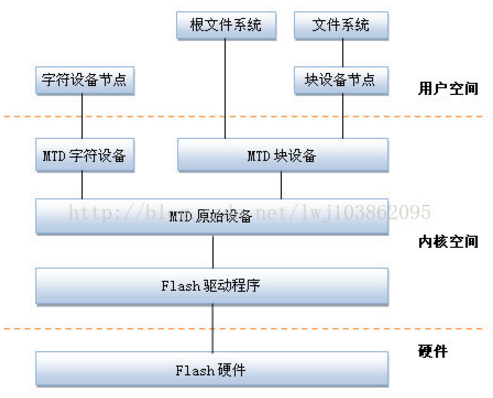
\includegraphics[keepaspectratio,width=0.5\textwidth,height=0.75\textheight]{img/mtd_struct.png}
\end{figure}
在上图中可以发现,MTD原始设备是对NandFlash封装的一层。下面主要分析原始设备层是如何使用NandFlash驱动,以及向上层提供了哪些封装函数

\section{MTD原始设备层}
操作NandFlash主要有三个动作,读/写/擦除。MTD原始设备在read/write/erase函数中会调用nand flash chip驱动的相应操作方法,而文件系统则可以直接使用原始设备层提供的read/write/erase去操作flash。
\clearpage
\subsection{主要数据结构分析}
struct mtd\_info就代表MTD原始设备层,这个结构体的函数是需要驱动开发人员实现的,实现这些函数比较简单,基本都是直接调用nand flash驱动的函数。
\begin{lstlisting}[language=C]
struct mtd_info {
	u_char type; //nor flash or nand flash(mlc/slc/tlc)
	uint32_t flags; //mtd-abi.h中定义它的属性值
	uint64_t size; //mtd设备大小,就是分区大小
	uint32_t erasesize; //block大小
	uint32_t writesize; //最小写单位,对于nandflash就是PageSize(或subPageSize)
	uint32_t writebufsize; //基本未使用,writebufsize可以减少向flash写入次数
	uint32_t oobsize; //OOB字节数,spare space size
	uint32_t oobavail; //可用OOB字节数
	unsigned int erasesize_shift; //默认0
	unsigned int writesize_shift; //默认0
	unsigned int erasesize_mask;  //默认0
	unsigned int writesize_mask;  //默认0
	unsigned int bitflip_threshold; //bitflip数超过这个值,就会报EUCLEAN错误,这个值可以通过sysfs修改
	const char *name; //mtd名字,一般就是分区名cat /proc/mtd读出来的
	int index; //不重要
	struct nand_ecclayout *ecclayout; //ecc在oob中布局,根据硬件得到
	unsigned int ecc_step_size; //一次对多少字节进行校验计算,一般是256或512字节
	unsigned int ecc_strength; //可校准bitflip位数
	int numeraseregions; //不同的erasesize区域数目,通常都是1
	struct mtd_erase_region_info *eraseregions;
	int (*_erase) (struct mtd_info *mtd, struct erase_info *instr); //块擦除函数
	... ...
	int (*_read) (struct mtd_info *mtd, loff_t from, size_t len,
		      size_t *retlen, u_char *buf); //读page函数
	int (*_write) (struct mtd_info *mtd, loff_t to, size_t len,
		       size_t *retlen, const u_char *buf); //写page函数
	int (*_panic_write) (struct mtd_info *mtd, loff_t to, size_t len,
			     size_t *retlen, const u_char *buf);
	int (*_read_oob) (struct mtd_info *mtd, loff_t from,
			  struct mtd_oob_ops *ops); //带oob读函数
	int (*_write_oob) (struct mtd_info *mtd, loff_t to,
			   struct mtd_oob_ops *ops); //带oob写函数
	... ...
	void (*_sync) (struct mtd_info *mtd);
	int (*_lock) (struct mtd_info *mtd, loff_t ofs, uint64_t len); //nandflash支持设备独占访问才能定义
	int (*_unlock) (struct mtd_info *mtd, loff_t ofs, uint64_t len);//nandflash解锁
	int (*_is_locked) (struct mtd_info *mtd, loff_t ofs, uint64_t len);
	int (*_block_isreserved) (struct mtd_info *mtd, loff_t ofs);
	int (*_block_isbad) (struct mtd_info *mtd, loff_t ofs); //坏块判断函数
	int (*_block_markbad) (struct mtd_info *mtd, loff_t ofs); //使用中出现坏块时的标记函数
	int (*_suspend) (struct mtd_info *mtd);
	void (*_resume) (struct mtd_info *mtd);
	int (*_get_device) (struct mtd_info *mtd);
	void (*_put_device) (struct mtd_info *mtd);
	struct backing_dev_info *backing_dev_info;
	struct notifier_block reboot_notifier;
	struct mtd_ecc_stats ecc_stats;
	int subpage_sft;
	void *priv;
	struct module *owner;
	struct device dev;
	int usecount;
};

\end{lstlisting}
\clearpage
struct nand\_chip结构体代表的是flash驱动,它是直接与硬件通信的,因此nand\_chip中的需要用到的函数都是由驱动开发人员实现。nand chip也不必使用MTD自带的struct nand\_chip,驱动开发自己定义,然后自己实现也是可以的,高通自定义的为struct msm\_nand\_chip。
\begin{lstlisting}[language=C]
struct nand_chip {
	void __iomem *IO_ADDR_R; //读写8根IO线的地址
	void __iomem *IO_ADDR_W;
	uint8_t (*read_byte)(struct mtd_info *mtd); //读flash单一字节
	u16 (*read_word)(struct mtd_info *mtd);
	void (*write_byte)(struct mtd_info *mtd, uint8_t byte);
	void (*write_buf)(struct mtd_info *mtd, const uint8_t *buf, int len);
	void (*read_buf)(struct mtd_info *mtd, uint8_t *buf, int len);
	void (*select_chip)(struct mtd_info *mtd, int chip);
	int (*block_bad)(struct mtd_info *mtd, loff_t ofs, int getchip);
	int (*block_markbad)(struct mtd_info *mtd, loff_t ofs);
	void (*cmd_ctrl)(struct mtd_info *mtd, int dat, unsigned int ctrl);
	int (*init_size)(struct mtd_info *mtd, struct nand_chip *this,
			u8 *id_data);
	int (*dev_ready)(struct mtd_info *mtd);
	void (*cmdfunc)(struct mtd_info *mtd, unsigned command, int column,
			int page_addr);
	int(*waitfunc)(struct mtd_info *mtd, struct nand_chip *this);
	int (*erase)(struct mtd_info *mtd, int page);
	int (*scan_bbt)(struct mtd_info *mtd);
	int (*errstat)(struct mtd_info *mtd, struct nand_chip *this, int state,
			int status, int page);
	int (*write_page)(struct mtd_info *mtd, struct nand_chip *chip,
			uint32_t offset, int data_len, const uint8_t *buf,
			int oob_required, int page, int cached, int raw);
	int (*onfi_set_features)(struct mtd_info *mtd, struct nand_chip *chip,
			int feature_addr, uint8_t *subfeature_para);
	int (*onfi_get_features)(struct mtd_info *mtd, struct nand_chip *chip,
			int feature_addr, uint8_t *subfeature_para);
	int (*setup_read_retry)(struct mtd_info *mtd, int retry_mode);
	int chip_delay;
	unsigned int options;
	unsigned int bbt_options;
	int page_shift;
	int phys_erase_shift;
	int bbt_erase_shift;
	int chip_shift;
	int numchips;
	uint64_t chipsize;
	int pagemask;
	int pagebuf;
	unsigned int pagebuf_bitflips;
	int subpagesize;
	uint8_t bits_per_cell;
	uint16_t ecc_strength_ds;
	uint16_t ecc_step_ds;
	int onfi_timing_mode_default;
	int badblockpos;
	int badblockbits;
	int onfi_version;
	int jedec_version;
	union {
		struct nand_onfi_params	onfi_params;
		struct nand_jedec_params jedec_params;
	};
	int read_retries;
	flstate_t state;
	uint8_t *oob_poi;
	struct nand_hw_control *controller;
	struct nand_ecc_ctrl ecc;
	struct nand_buffers *buffers;
	struct nand_hw_control hwcontrol;
	uint8_t *bbt;
	struct nand_bbt_descr *bbt_td;
	struct nand_bbt_descr *bbt_md;
	struct nand_bbt_descr *badblock_pattern;
	void *priv;
};

\end{lstlisting}
























